\chapter{序論}
\label{chap:intro}
\fancyhf{}
\rhead{\thepage}
\lhead{第\ref{chap:intro}章 序論}
\cfoot{\thepage}

本章では,本論文の背景,研究目的および本論文の構成について述べる.


\section{研究の背景}

\subsection{教育の個人最適化の重要性}
% 導入:学習の個人最適化
近年,教育とITの融合が進む中で,「アダプティブラーニング」という言葉が注目されている.
個人に最適化された学習内容の自動提供を実現するもので,そのシャキ的影響の大きさからアメリカを中心に注目が集まっており,
関連するスタートアップや大学での研究に,多額の資金が投入されている\cite{piccioli2014learning}.


学習内容を個人に最適化するという考え方は,決して新しいものではない.
現在の学校教育では,一人の教師が,複数の生徒に対して同時に教育する形態が一般的であるが,
学習の速度や教科による得手不得手は人それぞれであり,
同じ教育を施しても,十分な理解ができず,つまずいてしまう生徒もいる.
そのため,習熟が遅れている生徒に補習を行い,つまずいている原因を解明して克服する手助けをするように,
生徒の学習状態を考慮して学習内容を設計する試みは,常に行われてきており,
そうした指導の調整が巧みな教師は「腕のいい」教師として評価されてきた.

しかしこうした方法では,
習熟の遅い生徒を援助することに重きが置かれるため,習熟が周りより早い生徒への対応は後回しにされることが多く,発展的な学習機会や知的好奇心の向上を妨げることに加え,
現実的な時間と労力を考慮すると,全ての生徒に個別に対応することは困難である.


より個別化された教育を受ける手段として,個別指導形式の塾や家庭教師,通信教育なども利用される.
生徒一人一人に教師がつき,生徒の習熟度合いを考慮して教育を設計できるため,
習熟の早い生徒も発展的な内容を学習することが可能で,
また,誰かが優先された誰かが後回しにされるということもなく,
学習内容を最適化するという目的の上では,より望ましい.

しかし,このように,教育の粒度を細かくし,個人最適化を図ろうとするほど,
教師一人あたりが担当できる生徒の数が減ることによる人材的・金銭的負担や,
教師ごとの指導能力の違いなどの問題に直面する.
結局,このような教師のマンパワーに依存した方法では,
誰もが平等に最適な教育を受けるという目的を達成するには,障壁が残る.


\subsection{オンライン教育サービスの普及と学習効果分析の発展}
% 背景1:オンライン学習サービスを利用した個人最適化,データ蓄積に伴う学習効果分析の進展
こうした問題意識から,最適な学習内容を自動で提供することを目的としてアダプティブラーニングの考え方が登場したが,
その原動力となっているのが,オンライン教育サービスの普及である.

オンライン教育サービスとは,
従来の学校の教室で,一人の教師が複数の生徒に対して同時に教育する形態と異なり,
PCやモバイル端末を通じて,
オンライン上で提供される学習コンテンツを,生徒が各自で利用するサービスを指す.

オンライン教育サービスの一つであるMassive Open Online Courses(MOOCs)\cite{mcauley2010mooc, pappano2012year,siemens2013massive}は,
多様な分野や難易度の講義から,時間や場所を問わずに,生徒が自分のペースで学習したいものを選択して学習できるというもので,
従来の教育が抱える,全ての生徒が,自身の習熟度合いに沿った教育を受けられないという問題を解決するものとして,活用が期待されている.
例えば,世界最大級のMOOCsの一つであるCoursera\footnote{\url{https://www.coursera.org/}}は,
2017年1月の時点で,
29の国にまたがる148の教育機関とパートナーシップを結び,
コンピュータサイエンス,数学や論理,社会科学などに関する1600以上の講座を,2200万人以上に提供している.
日本では2013年2月に東京大学がCourseraに,2013年5月に京都大学がedX\footnote{\url{https://www.edx.org/}}に参加を表明したことから普及し,
2013年11月には日本版のMOOCsとしてJMOOC\footnote{\url{https://www.jmooc.jp/}}が設立されるなど,
国内外でMOOCsの利用が拡大している.

多様な講座を多くの人に提供するMOOCs以外にも,
より個人の学習過程をサポートすることを目的として設計された,
Intelligent Tutoring System(ITS)と呼ばれるオンライン自動学習支援システムの利用も拡大している.
世界最大級のITSであるKnewton\footnote{\url{https://www.knewton.com/}}では,
生徒の学力や理解度と,学ぶべき対象をマッピングすることで、
生徒に最適な学習過程を設計し,
かつ生徒の学習の進捗に応じてその過程を動的に変化させる仕組みを有している\cite{upbin2012knewton}.

近年ではITSとMOOCsの融合も進んでおり\cite{aleven2015beginning},
オンライン教育サービスの利用が世界中で拡大している.

日本でも,生徒が自宅でオンライン教育サービスを用いて知識を学び,
学校ではより参加型のディスカッションを行うという「反転学習」
の試みが提唱されており,オンライン教育サービスが社会に与える影響は今後さらに大きくなっていくといえる\cite{lage2000inverting, 重田勝介2014反転授業}.


% 背景1−B:オンライン教育サービスによるビッグデータの蓄積と活用
さらに,オンライン教育サービスは,新たな学習形態を提供するのみにとどまらず,
これまで困難であった,大規模な学習効果分析を可能にするプラットフォームとして期待されている.

オンライン上で提供された講義を生徒が学習する際に,その学習行動ログをデータとして蓄積することが可能なため,
そうして蓄積された多様な学習者の大規模な学習行動ログから,多様な学習効果の分析が可能になった.
特に,演習問題の回答ログは,その問題が問う知識を学習者が獲得しているか否かを表すため,知識獲得の分析に利用できる\cite{corbett1994knowledge}.
例えば,生徒の問題回答ログを利用して知識獲得の予測を行った研究\cite{machardy2015toward}は,
有名なMOOCsの一つであるKhan Academy\footnote{\url{https://www.khanacademy.org/}}に蓄積された100万件以上の問題回答ログを使用しており,
教育の分野における大規模データを適用した分析の一つである.

生徒が個人で利用するというオンライン教育サービスの特性によって,
このような研究成果を元に,学習コンテンツを個人に最適化して提供することが容易になったため,
学習の個人最適化を進める運動は,急速に活発化している.


\subsection{深層学習の躍進}
% 背景2:深層学習の高まり
一方,近年,教育に限らない多くの研究領域で,深層学習が注目されている.

従来の機械学習では,人間が問題の特徴を捉えて素性を設計する必要があったが,
深層学習では,目的に応じた素性を,データから自動で学習することが可能になり,
画像認識\cite{schroff2015facenet,szegedy2014going},
音声認識\cite{hinton2012deep, bahdanau2015end},
機械翻訳\cite{sutskever2014sequence, dong2015multi}等,
多様な研究領域で飛躍的な進展が報告がされている.

特に,直近の一年間だけでも
画像から動画を生成する研究\cite{vondrick2016generating}や,
会話を人間と同程度に認識できるとする音声認識の研究\cite{xiong2016achieving},
一部の欧米言語間の文レベルで,ほぼ人間と同等に正確な翻訳を実現したとする機械翻訳の研究\cite{wu2016google}なども報告されており,
深層学習によって,日々驚異的な成果が生み出されている.

また,2016年3月に人間のプロを倒したことで一躍有名になった,Google Deep Mindが開発したコンピュータ囲碁プログラムの「AlphaGo」\cite{silver2016mastering}は,
過去の人間が打った大量の棋譜に深層学習を適用した後,コンピュータ同士の対局による強化学習を通して,
今後10年は不可能と言われていた,人間のプロを打ち負かすほどの棋力を獲得した.
AlphaGoは,過去の対極である棋譜の分析によって人間を真似ただけでなく,
それまで人間が考えつかなかったような手を学習しており,囲碁界に衝撃を与えている.
このように,深層学習は,人間が認識できないようなデータの複雑な特徴を捉えることで,
これまで人間が作り上げてきた概念を,大きく塗り替える可能性を秘めている.


こうした深層学習の技術は,オンライン教育サービスに蓄積されたデータを元にした,学習効果の分析にも活用が期待されている.

特に,生徒の知識状態をモデリングし,知識獲得を予測するKnowledge Tracingの研究は,
生徒の知識状態を正しく把握することで,最適な学習内容を特定することにつながるため,以前から研究が盛んだったが,
深層学習の適用により大きく進展した.
Piechらが発表した,Knowledge Tracingに深層学習を活用するDeep Knowledge Tracingという手法では,
時系列分析でよく用いられる深層学習モデルであるRecurrent Neural Networks\cite{williams1989learning}を活用することで,
高い性能で知識獲得を予測できること,
また,予測モデルを分析することで知識間関係をネットワークとして抽出できることが報告されている\cite{piech2015deep}.


しかし,こうした知識獲得予測に深層学習を適用する研究においては,ある問題が存在する.
知識獲得を予測するアルゴリズムの部分には深層学習を適用しているものの,
素性となる「知識」は,事前に人間が作成した知識分類によって定義されており,
人間が設計した素性を利用する旧来の状況から脱していない.
人間が作成した分類というのは,
「知識の体系はこうなっているはずだ」ないしは「この体系に基づいて教えられることが望ましい」という専門家の仮説や理論に基づいて作られたものである.
そのため,人間にとっての可読性は高いとしても,
実際の生徒の知識獲得の過程を定量的に分析した上で,知識獲得の予測性が最適化されているという根拠はない.

今日多様な分野で成果を生んでいる,データから特徴を自動で学習できる深層学習を活用すれば,
人間が認識できないような,知識獲得の過程を反映し,予測を最適化するような知識分類を学習できる可能性は高く,
生徒の学習効率を最適化するという最終的な目標を真に達成するには,
知識分類自体も深層学習によって最適化される必要があるといえる.

以上の問題意識に基づいた,既存研究との本研究の差分のイメージを図\ref{fig:problem}に示す.
\begin{figure}[htb]
\begin{center}
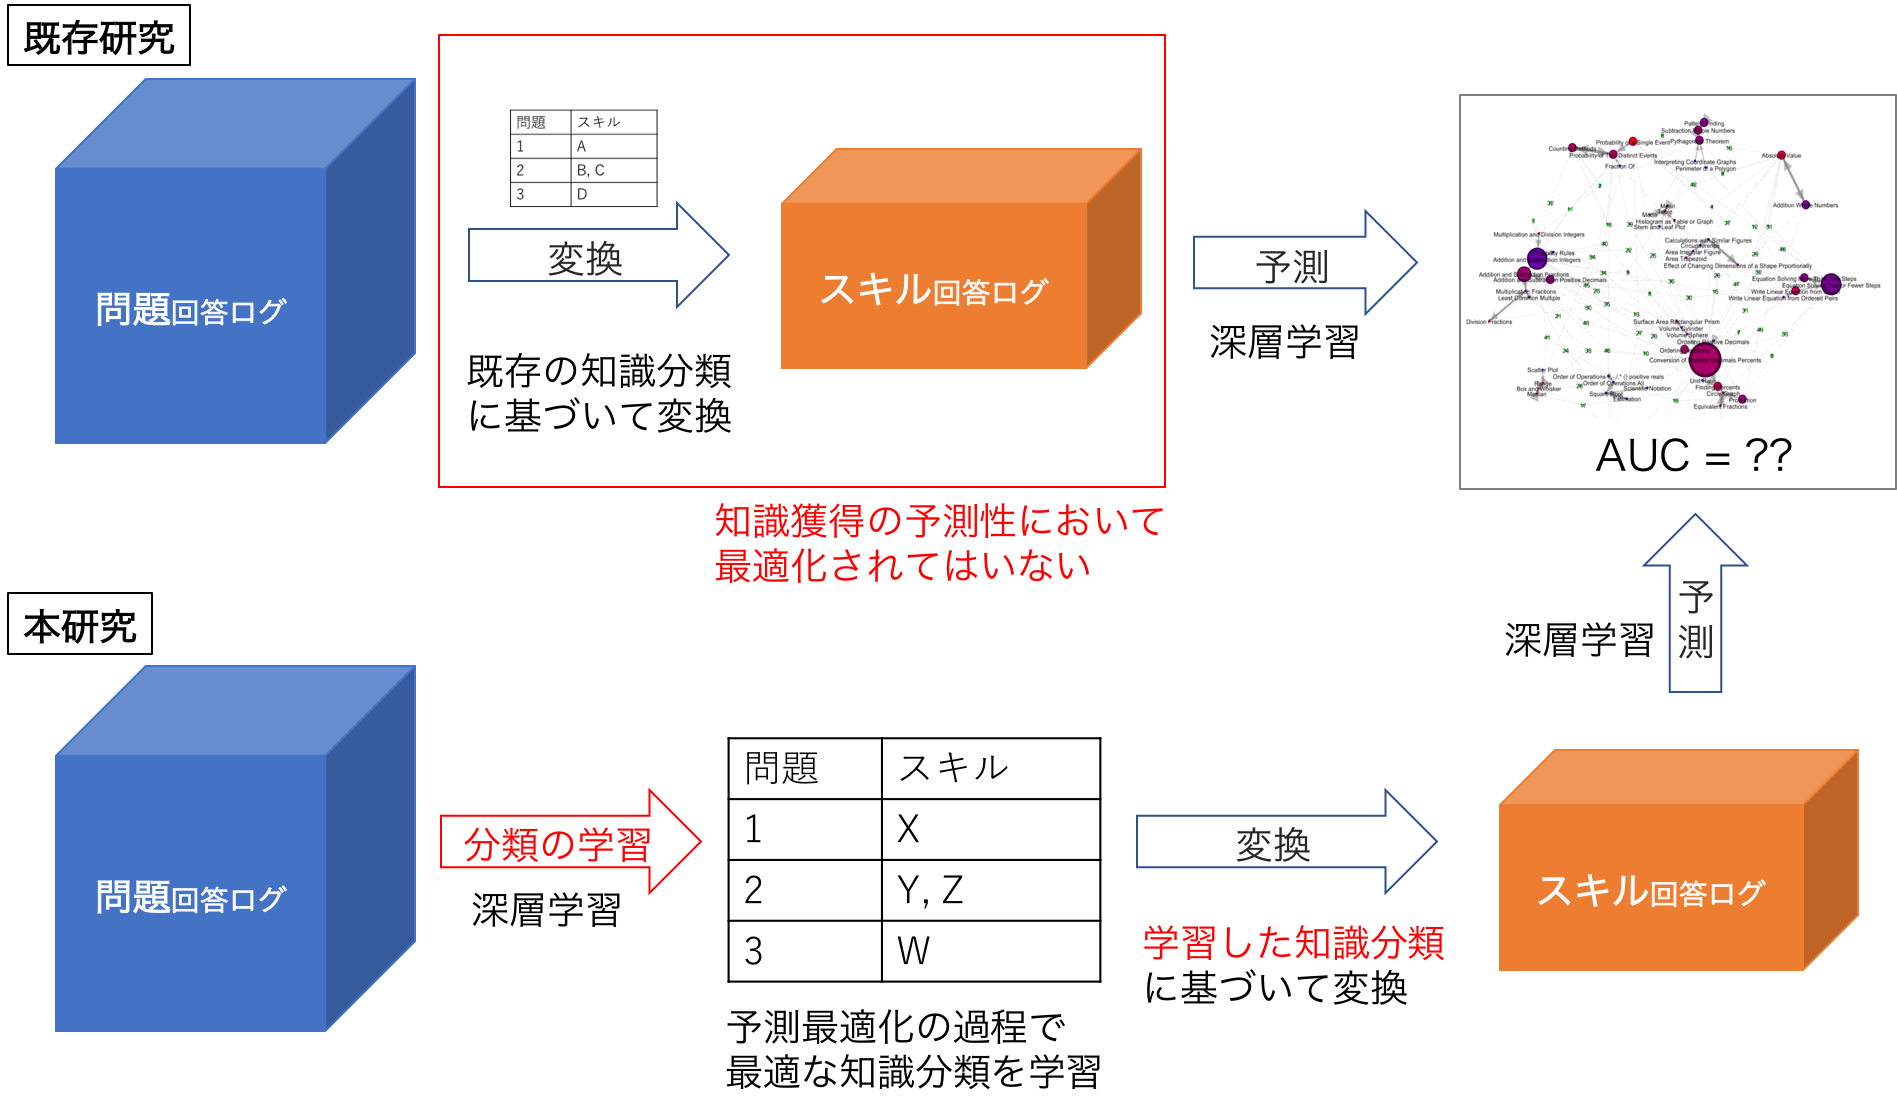
\includegraphics[width=350pt]{./img/problem.png}
\end{center}
\caption{既存研究と本研究の差分のイメージ}
\label{fig:problem}
\end{figure}


\vvspace
以上,本研究の背景について述べた.
次に,上記の背景を踏まえた研究目的について説明する.

\section{研究目的}
本研究では,
現在の知識獲得予測に用いられている,専門家が作成した知識分類は,人間の複雑な知識獲得過程を表現する上では最適化されていない,という仮定に立ち,
下記を検証することを目的とする.

\begin{itemize}
\item 深層学習によって抽出した知識分類を用いることで,専門家が作成した知識分類を用いる場合よりも,高い精度で知識獲得予測を行うことができる.
\end{itemize}

本論文では,専門家による事前の知識分類を所与のものとせずに,
問題の回答ログデータのみを深層学習に適用し,回答正誤予測を行う過程で,
その予測性を最適化する知識分類を抽出することを目的としている.

従来,専門家が事前に分類することが必要であった生のデータから,
予測性において最適な分類を深層学習によって自動で抽出できることを明らかにすることは,
既存の学問体系やカリキュラム設計の再構築につながるだけでなく,
人間の知識状態の推移するメカニズムを解明することにもつながり,
学術的な意義が大きいと考える.


\vvspace
以上,本研究の目的について述べた.
次に,背景と目的を踏まえて本論文の構成について述べる.



\section{本論文の構成}
以降の本論文の構成について述べる.

% 差分を明確にし,研究価値をあきらかにするために,関連情報与える.
2章では,関連研究について述べる.

知識獲得予測の関連研究を俯瞰し,
周辺概念を整理することで,本研究の学術的位置づけを明確にする.


% 差分を明確にし,その差分が重要であることを示す.分析手法
3章では,分析手法について述べる.
生徒の知識獲得を予測する過程で知識分類を抽出し,また,抽出された知識分類を分析する手法について説明する.
まず,分析手法全体の流れを概説し,手法全体が3つの要素から構成されることを述べる.


4章では,
実験で用いるデータセットについて述べる.
3章で述べたデータセットとしての要件を満たす,
オンライン教育サービスにおける生徒の学習回答ログである,2つのデータセットを紹介し,
本研究に適用するための事前の処理を説明する.


5章では,実験について述べる.
3つのブロックに分けられる実験について,各実験の設定を述べた後,
実験結果について述べる.

実験結果においては,
提案手法によって抽出された知識分類を用いることで,既存の知識分類を用いた場合よりも高い精度で知識獲得を予測できることを確認し,
予測性能が最適化された知識分類が,Deep Knoeldge Tracingの過程で抽出されたことを定量的に示す.

さらに,抽出された知識分類について,
既存の知識分類との比較や,デートセットごとの比較をすることで,
定量的・定性的に解釈する.


6章では,実験結果を踏まえた考察を述べる.

まず,本研究で用いた手法や抽出された知識分類について,
実験結果を踏まえて,その性質を考察し,実際の教育現場への適用について述べる.

また,
本研究で用いた分析手法の,多様なデータへの適用可能性について議論し,
教科によらず知識構造を分析できる可能性があること,教科によって抽出される知識分類の性質が異なる可能性があること,
一方で,複合的な学問や専門性の高い学問については,適用可能性の検証実験が必要であることを述べる.
さらに,本研究で用いた分析手法が,教育学以外の分野にも応用できる可能性を持つことを論じる.


最後に,7章で結論を述べる.



\vvspace
以上,序論について述べた.
次に,先行研究について述べる.


